% !TEX program = lualatex
\documentclass[11pt]{article}

% -------- LuaLaTeX : polices et langue --------
\usepackage{fontspec}
\setmainfont{Latin Modern Roman}
\setsansfont{Tex Gyre Heros}
%\renewcommand{\familydefault}{\sfdefault} % force le sans serif par défaut
\usepackage{polyglossia}
\setdefaultlanguage{french}

% -------- Mise en page --------
\usepackage[a4paper,margin=1cm]{geometry}
\usepackage{multicol}
\usepackage{fancyhdr}
\pagestyle{empty}
\usepackage[most]{tcolorbox}

% -------- Mathématiques --------
\usepackage{amsmath,amssymb,mathtools}
\usepackage{icomma}
% \sisetup{locale=FR}

\usepackage{enumitem}
\setlist[itemize]{left=0pt}
\setlist[enumerate]{left=0pt, label=\textbf{\arabic*}.}

\usepackage{ProfCollege}
\usepackage{ProfMaquette}

\usepackage{tabularray}

% -------- Divers --------
\setlength{\parindent}{0pt}

\begin{document}

\begin{Maquette}[Fiche]{Theme=Agrandissement et réduction, Niveau=Troisième}

\begin{exercice}
   Tom a inséré une image dans un fichier de traitement de texte. L’image étant trop petite, il l’a donc agrandie. Quelle est à présent la hauteur de l’image ?
   \begin{center}
    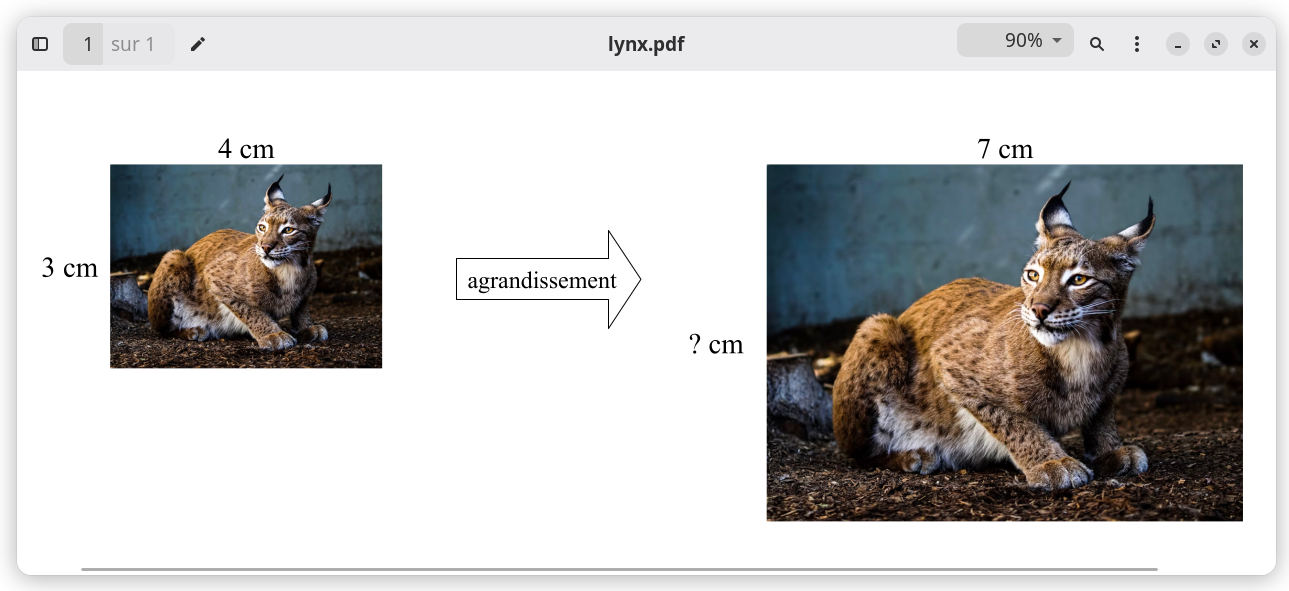
\includegraphics[width=.9\linewidth]{Images/Exercice1-Lynx.png}
   \end{center}
\end{exercice}

\begin{multicols}{2}

   \begin{exercice}
      \begin{enumerate}
         \item Léo pense que pour que deux figures soient dans une situation d’agrandissement/réduction, il suffit qu’elles aient les mêmes angles. Démontre que cela est faux en proposant un \emph{contre-exemple} à l’aide de deux quadrilatères.
         \item Anna pense qu’il suffit qu’elles aient des longueurs proportionnelles. Démontre que cela est également faux.
      \end{enumerate}
      
   \end{exercice}

   \begin{exercice}
      On agrandit un triangle rectangle :
      \begin{center}
         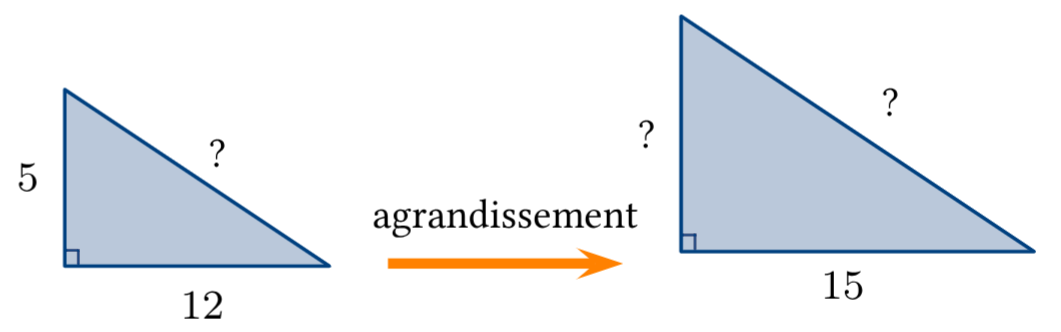
\includegraphics[width=.9\linewidth]{Images/Exercice3.png}
      \end{center}
      \begin{enumerate}
         \item Quel est le rapport d’agrandissement ?
         \item Calcule les longueurs manquantes.
      \end{enumerate}
   \end{exercice}
\end{multicols}

\end{Maquette}

\end{document}
